\chap{ Adders, Subtractors, and Multipliers}

\section{Introduction}
The purpose of this exercise is to examine arithmetic circuits that add, subtract, and multiply numbers. Each circuit will be described in Verilog and implemented on an Intel FPGA DE10-Lite, DE0-CV, DE1-SoC, or DE2- 115 board.
\section{Part IV}
\begin{itemize}
    \item [] \textbf{REQUIREMENT}
        \begin{enumerate}
            \item In Part III, an array multiplier was implemented using full adder modules. At a higher level, a row of full adders functions as an n-bit adder and the array multiplier circuit can be represented as shown in Figure 5.
                 \begin{figure}[h]
                    \centering
                    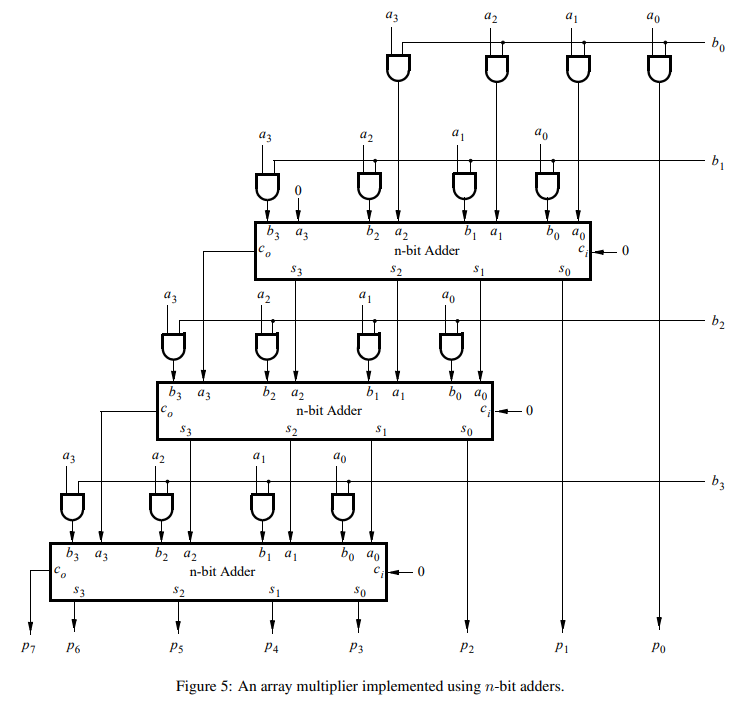
\includegraphics[scale = 0.75]{source/picture/Lab6/Lab6_4_0.png}
                \end{figure}
\clearpage
            \item Each n-bit adder adds a shifted version of A for a given row and the partial product of the row above. Abstracting the multiplier circuit as a sequence of additions allows us to build larger multipliers. The multiplier should consist of n-bit adders arranged in a structure shown in Figure 5. Use this approach to implement an 8 x 8 multiplier circuit with registered inputs and outputs, as shown in Figure 6.
                \begin{figure}[h]
                    \centering
                    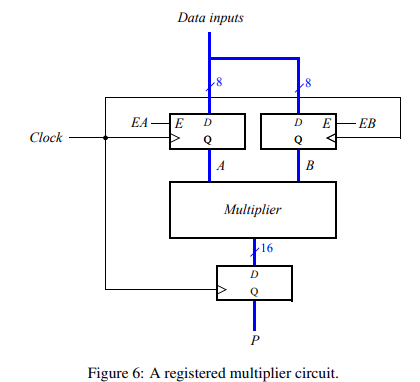
\includegraphics[scale = 0.9]{source/picture/Lab6/Lab6_4_1.png}
                \end{figure}
        \end{enumerate}
    \item [] \textbf{SOLUTION}
        \begin{lstlisting}[language=verilog]
module part4(CLK, IN,EA,EB,P);
	input		CLK, EA, EB;
	input		[7:0]IN;
	output	[15:0]P;
	
	wire	[7:0] A,B;
	wire	[15:0]SUM;
	wire	[7:0] adder1_in0, adder1_in1;
	wire	[7:0] adder2_in0, adder2_in1;
	wire 	[7:0] adder3_in0, adder3_in1;
	wire	[7:0] adder4_in0, adder4_in1;
	wire	[7:0] adder5_in0, adder5_in1;
	wire 	[7:0] adder6_in0, adder6_in1;
	wire	[7:0] adder7_in0, adder7_in1;

	D_FF	inputa_ff (.CLK(CLK), .EN(EA), .D(IN),  .Q(A));
	D_FF	inputb_ff (.CLK(CLK), .EN(EB), .D(IN),  .Q(B));
	D_FF	output_ff (.CLK(CLK), .EN(1),  .D(SUM), .Q(P));
	
	multiply_Nx1	inst0		(.A(A), .B(B[0]),      .P({adder1_in0[6:0],SUM[0]}));
	multiply_Nx1	inst1		(.A(A), .B(B[1]), .P(adder1_in1));
	multiply_Nx1	inst2		(.A(A), .B(B[2]), .P(adder2_in1));
	multiply_Nx1	inst3		(.A(A), .B(B[3]), .P(adder3_in1));
	multiply_Nx1	inst4		(.A(A), .B(B[4]), .P(adder4_in1));
	multiply_Nx1	inst5		(.A(A), .B(B[5]), .P(adder5_in1));
	multiply_Nx1	inst6		(.A(A), .B(B[6]), .P(adder6_in1));
	multiply_Nx1	inst7		(.A(A), .B(B[7]), .P(adder7_in1));
	
	sumNbits adder1 (.A(adder1_in0), .B(adder1_in1), .C_IN(0) ,.SUM({adder2_in0[2:0],SUM[1]}) ,.C_OUT(adder2_in0[3]));
	sumNbits adder2 (.A(adder2_in0), .B(adder2_in1), .C_IN(0) ,.SUM({adder3_in0[2:0],SUM[2]}) ,.C_OUT(adder3_in0[3]));
	sumNbits adder3 (.A(adder3_in0), .B(adder3_in1), .C_IN(0) ,.SUM({adder4_in0[2:0],SUM[3]}) ,.C_OUT(adder4_in0[3]));
	sumNbits adder4 (.A(adder4_in0), .B(adder4_in1), .C_IN(0) ,.SUM({adder5_in0[2:0],SUM[4]}) ,.C_OUT(adder5_in0[3]));
	sumNbits adder5 (.A(adder5_in0), .B(adder5_in1), .C_IN(0) ,.SUM({adder6_in0[2:0],SUM[5]}) ,.C_OUT(adder6_in0[3]));
	sumNbits adder6 (.A(adder6_in0), .B(adder6_in1), .C_IN(0) ,.SUM({adder7_in0[2:0],SUM[6]}) ,.C_OUT(adder7_in0[3]));
	sumNbits adder7 (.A(adder7_in0), .B(adder7_in1), .C_IN(0) ,.SUM(SUM[14:7]) 		  ,.C_OUT(SUM[15]));
	
	defparam inputa_ff.n_bits = 8;
	defparam inputb_ff.n_bits = 8;
	defparam output_ff.n_bits = 16;
	
	defparam inst0.n_bits = 8;
	defparam inst1.n_bits = 8;
	defparam inst2.n_bits = 8;
	defparam inst3.n_bits = 8;
	defparam inst4.n_bits = 8;
	defparam inst5.n_bits = 8;
	defparam inst6.n_bits = 8;
	defparam inst7.n_bits = 8;
	
	defparam	adder1.n_bits = 8;
	defparam	adder2.n_bits = 8;
	defparam	adder3.n_bits = 8;
	defparam	adder4.n_bits = 8;
	defparam	adder5.n_bits = 8;
	defparam	adder6.n_bits = 8;
	defparam	adder7.n_bits = 8;
endmodule
        \end{lstlisting}
   \item[]\textbf{VERIFICATION}
        \begin{figure}[h]
            \centering
            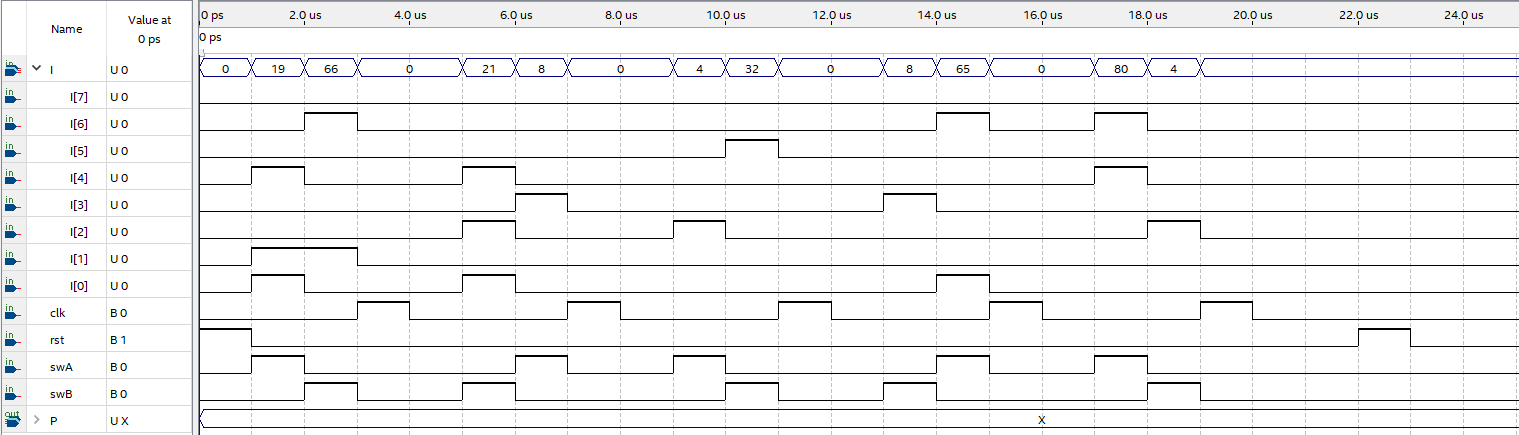
\includegraphics[width=\textwidth]{source/picture/Lab6/Lab6 _4.png}
            \caption{Simulation Result}
        \end{figure}
\end{itemize}
\clearpage
\section{Part 5}
\begin{itemize}
    \item []\textbf{REQUIREMENT}
        \begin{enumerate}
            \item Part IV showed how to implement multiplication A × B as a sequence of additions, by accumulating the shiftedversions of A one row at a time. Another way to implement this circuit is to perform addition using an adder tree. An adder tree is a method of adding several numbers together in a parallel fashion.
                \begin{figure}[h]
                    \centering
                    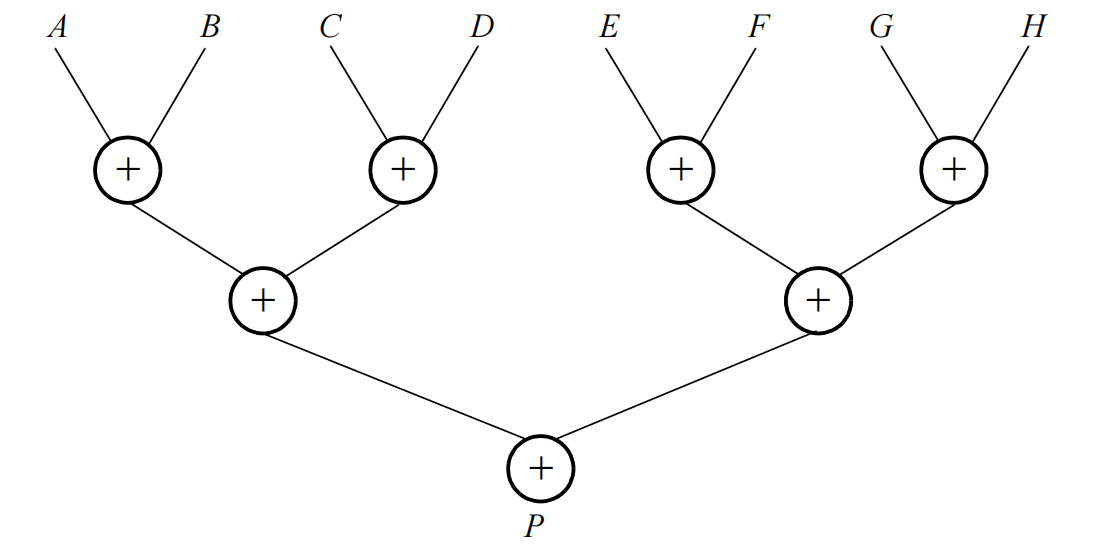
\includegraphics[width=\textwidth]{source/picture/Lab6/lab6_adder_treee.png}
                    \caption{Adder tree}
                \end{figure}
            \item In this part you are to implement an 8 x 8 multiplier circuit by using the adder-tree approach. Inputs A and B, as well as the output P should be registered as in Part IV
        \end{enumerate}
    \item []\textbf{SOLUTION}
        \begin{itemize}
            \item []In this part we try to implement multiplication by adder tree or we will add in parallel rather than sequence additions
            \item []So firstly I create \textbf{add\_8bit} module with use to calculate the sum of two numbers 8 bit.
                \begin{figure}[h]
                    \centering
                    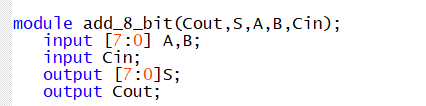
\includegraphics[width=\textwidth]{source/picture/Lab6/Lab6_add8bit.png}
                    \caption{Module add\_8\_bits}
                \end{figure}
            \item []Then create \textbf{MUL} module but now use parallel adding or (adder tree) so with A, B 8 bits number I will separate it into 8 layers and extern each layer to 8 bit.
                \begin{figure}[h]
                    \centering
                    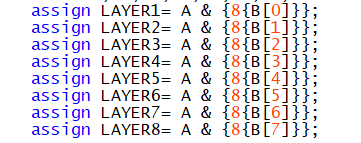
\includegraphics[width=\textwidth]{source/picture/Lab6/Lab6_mul.png}
                    \caption{Module MUL}
                \end{figure}
            \item []After having separated layers represent A,B,C … in picture then I do add operations like the image above.
                \begin{figure}[h]
                    \centering
                    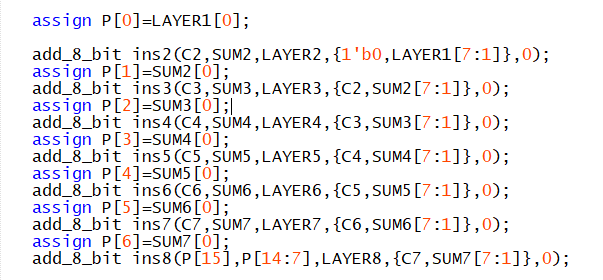
\includegraphics[width=\textwidth]{source/picture/Lab6/Lab6_rest.png}
                    \caption{Main program}

                \end{figure}
        \end{itemize}   
\end{itemize}
\clearpage
